\documentclass[12pt,letterpaper]{article}
\usepackage{graphicx}
\usepackage{textcomp}
\usepackage{natbib}
\usepackage{setspace}
\usepackage[margin=1in]{geometry}
\usepackage{color}
\usepackage[reqno]{amsmath}
\usepackage{amsthm}
\usepackage{fancyvrb}
\usepackage{amssymb}
\usepackage[all]{xy}
\usepackage{endnotes}
\usepackage{lscape}
\usepackage{float}
\usepackage{hyperref}
\usepackage[compact]{titlesec}
\usepackage{dcolumn}
\usepackage{tikz}
\usetikzlibrary{arrows}
\usepackage{multirow}
\usepackage{xcolor}
\usepackage{url}
\usepackage{listings}

% Define code highlighting colors
\definecolor{codegreen}{rgb}{0,0.6,0}
\definecolor{codegray}{rgb}{0.5,0.5,0.5}
\definecolor{codepurple}{rgb}{0.58,0,0.82}
\definecolor{backcolour}{rgb}{0.95,0.95,0.92}

% Define code listing style
\lstdefinestyle{mystyle}{
	backgroundcolor=\color{backcolour},   
	commentstyle=\color{codegreen},
	keywordstyle=\color{magenta},
	numberstyle=\tiny\color{codegray},
	stringstyle=\color{codepurple},
	basicstyle=\footnotesize,
	breakatwhitespace=false,         
	breaklines=true,                 
	captionpos=b,                    
	keepspaces=true,                 
	numbers=left,                    
	numbersep=5pt,                  
	showspaces=false,                
	showstringspaces=false,
	showtabs=false,                  
	tabsize=2
}
\lstset{style=mystyle}

\title{Problem Set 1}
\date{Due: October 1, 2023}
\author{Applied Stats/Quant Methods 1}


\begin{document}
	\maketitle

	\section*{Instructions}
	\begin{itemize}
		\item Please show your work! You may lose points by simply writing in the answer. If the problem requires you to execute commands in \texttt{R}, please include the code you used to get your answers. Please also include the \texttt{.R} file that contains your code. If you are not sure if work needs to be shown for a particular problem, please ask.
		\item Your homework should be submitted electronically on GitHub.
		\item This problem set is due before 23:59 on Sunday October 1, 2023. No late assignments will be accepted.
		\item Total available points for this homework is 80.
	\end{itemize}
	
	\section*{Question 1 (40 points): Education}
	A school counselor was curious about the average IQ of the students in her school and took a random sample of 25 students' IQ scores. The following is the data set:
	
	\[ \{105, 69, 86, 100, 82, 111, 104, 110, 87, 108, 87, 90, 94, 113, 112, 98, 80, 97, 95, 111, 114, 89, 95, 126, 98\} \]
	
	\begin{enumerate}
		\item Find a 90\% confidence interval for the average student IQ in the school.
		\item Next, the school counselor was curious whether the average student IQ in her school is higher than the average IQ score (100) among all the schools in the country. Using the same sample, conduct the appropriate hypothesis test with $\alpha=0.05$.
	\end{enumerate}
	
	\section*{Question 1: Answers}
	
	\subsection*{Part 1.}
	
	First I analyzed the structure of the data and calculated it's mean, variance, standard deviation, standard error, and length for reference.  
	
	\begin{verbatim}
		
		str(y)
		mean(y) 
		var(y) 
		sd(y) 
		sd(y)/sqrt(length(y)) 
		length(y)
		
	\end{verbatim}
	
	The z-score for a 90 percent confidence interval = 1.645. Using the qnorm function I can calculate and assign the upper and lower bounds of the confidence interval. This method assumes a normally distributed population with a known standard deviation. It is also better used when the sample population size greater than 30. So in the case of our sample it will produce an incorrect result, but I will demonstrate it anyway.
	
	\begin{Verbatim}
{lower_95_n <- qnorm(0.05, 
	mean(y), 
	(sd(y)/sqrt(length(y))))
	print(lower_95_n)
	upper_95_n <- qnorm(0.95,
	mean(y),
	(sd(y)/sqrt(length(y))))
	print(upper_95_n)
}
	\end{Verbatim}
	
	Using this method the 90 percent confidence interval = 94.13283 - 102.7472.
	\vspace{5mm}
	
	Given the sample size is less than 30 (it is 25), and the exact population standard deviation is unknown it would be more accurate to assume the population follows a t distribution rather than a normal distribution. To calculate the 90 percent confidence interval using a t distribution we can use the t.test function, or do it manually.
	\vspace{5mm}
	
	To do it manually:
	
	\begin{Verbatim}
		#Calculate the degrees of freedom.
		
		df <- length(y)-1
		
		#Calculate the t-value.
		
		tvalue <- qt(0.95, df)
		
		#Calculate the margin of error.
		
		moe <- tvalue * (sd(y) / sqrt(length(y)))
		
		#Print results.
		
		lower_95t <- mean(y) - moe
		upper_95t <- mean(y) + moe
		
		print(lower_95t)
		print(upper_95t)
		
		#This gives us a 90 percent confidence interval of 93.95993-102.9201
	\end{Verbatim}
	
	Or to use the t.test function to get the same results we can use this line of code.
	\begin{verbatim}
	t.test(y, conf.level = 0.90, alternative = "two.sided")
    \end{verbatim}
The confidence interval using this method = 93.95993-102.92007
\vspace{10mm}

\subsection*{Part 2.}

Null hypothesis: The average student IQ in the teacher's school is the same as the average IQ score (100) among all the schools in the country.
\vspace{5mm}

H0: population mean = 100
\vspace{1mm}

Ha: population mean =/= 100
\vspace{1mm}

This is a two-sided test but it may be one-sided.
\vspace{5mm}

We have to calculate the p-value of the sample. Given the sample size we must use the t-score, rather than the z-score. (see page 118, Statistical Methods for the Social Sciences)
\vspace{5mm}

Calcuate sample mean, standard deviation, length for reference.
\begin{verbatim}
	mean(y)
	sd(y)
	length(y)
\end{verbatim}

Calculate the test statistic (TS).
\begin{Verbatim}
test_statistic <- (mean(y) - 100) / (sd(y) / sqrt(length(y)))
print(test_statistic)
\end{Verbatim}
Estimated standard error of the sample.
\begin{Verbatim}
	standarderror <- sd(y) / sqrt(length(y))
	print(standarderror)
\end{Verbatim}
Calculate the degrees of freedom
\begin{Verbatim}
     df <- length(y)-1
\end{Verbatim}
Calculate the P-Value
\begin{Verbatim}
	pvalue <- 1- pt(test_statistic, df)
	print(pvalue)
\end{Verbatim}
P-Value = 0.7215383

We could also use the t.test function to calculate the P-Value.
\begin{Verbatim}
	t_test_result <- t.test(y, mu = 100, alternative = "greater")
\end{Verbatim}
Giving us the same answer.
Given the level of significance (Alpha) is 0.05, the calculated P-Value is greater than Alpha, so we cannot reject the null hypothesis. The teacher cannot say for certain that her students have an IQ  higher on average than the average IQ score (100) among all the schools in the country.
	
	\section*{Question 2 (40 points): Political Economy}
	Researchers are curious about what affects the amount of money communities spend on addressing homelessness. The following variables constitute our data set about social welfare expenditures in the USA:
	
	\[
	\begin{tabular}{r|l}
		\texttt{State} & \emph{50 states in US} \\
		\texttt{Y} & \emph{per capita expenditure on shelters/housing assistance in state} \\
		\texttt{X1} & \emph{per capita personal income in state} \\
		\texttt{X2} & \emph{Number of residents per 100,000 that are "financially insecure" in state} \\
		\texttt{X3} & \emph{Number of people per thousand residing in urban areas in state} \\
		\texttt{Region} & \emph{1=Northeast, 2= North Central, 3= South, 4=West} \\
	\end{tabular}
	\]
	
	\begin{itemize}
		\item Please plot the relationships among \emph{Y}, \emph{X1}, \emph{X2}, and \emph{X3}? What are the correlations among them (you just need to describe the graph and the relationships among them)?
		\item Please plot the relationship between \emph{Y} and \emph{Region}? On average, which region has the highest per capita expenditure on housing assistance?
		\item Please plot the relationship between \emph{Y} and \emph{X1}? Describe this graph and the relationship. Reproduce the above graph including one more variable \emph{Region} and display different regions with different types of symbols and colors.
	\end{itemize}
	
	\section*{Question 2: Answers}
	
	\subsection*{Part 1.}
	Subset and name the relevant data.
	
	\begin{Verbatim}
		YX1X2X3 <- as.data.frame(expenditure[c("Y","X1","X2","X3")])
	\end{Verbatim}
	Use the pairs function in base R to create a scatter plot matrix of the four variables.
	\begin{Verbatim}
		pairs(YX1X2X3, main = "Expenditure Data")
	\end{Verbatim}
	
     For more detail we can use the car package to create a similar scatter plot matrix.
     
     Install the car package, Hannah Frank showed use this line of code to avoid an error message if the package is already installed.
     \begin{Verbatim}
     	if(!require(car)){
     		install.packages("car")
     		library(car)
     	}
     \end{Verbatim}
     
     Use scatterplotMatrix function from the car package to produce a scatter plot matrix of the four variables, with a line of best fit, and other details to illustrate the trends in the data. 
     
     \begin{Verbatim}
     	scatterplotMatrix(YX1X2X3, main = "Expenditure Data")
     \end{Verbatim}
     Which produced this scatter plot matrix:
\begin{center}
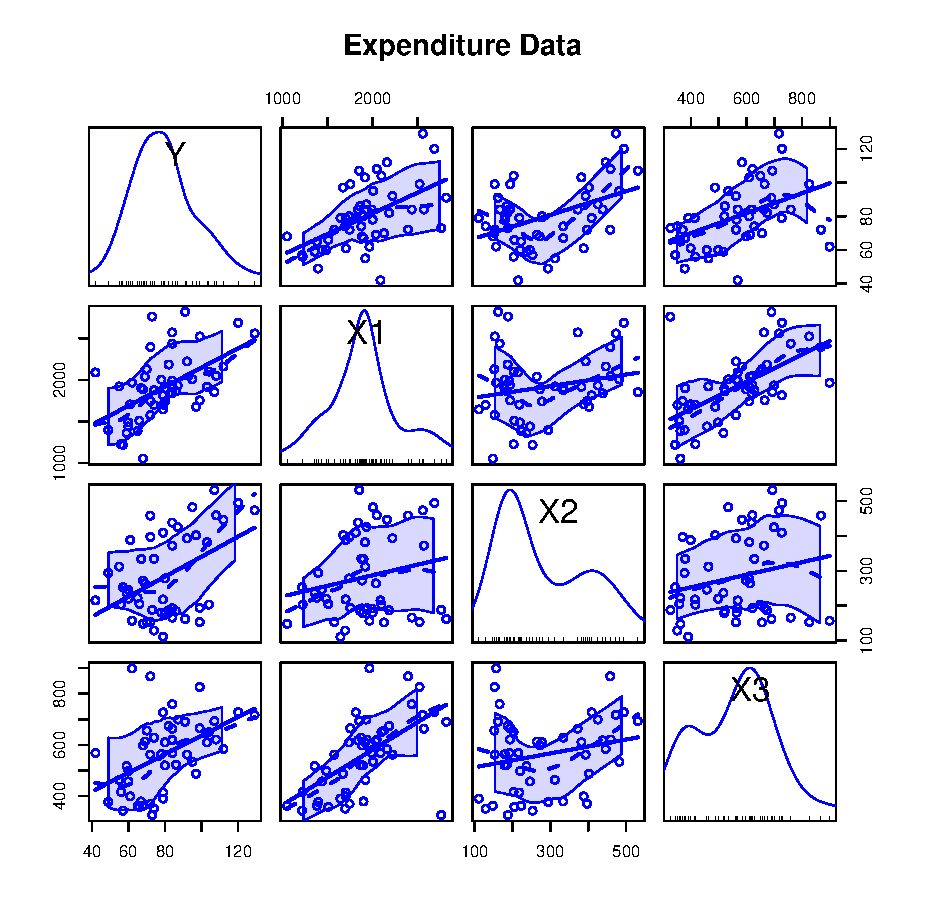
\includegraphics{Scatter_plot_Matrix_withtitle}\\
\end{center}
Based on this graphic we can see as per capita expenditure on housing goes up so do the amounts of all other variables.   
     \subsection*{Part 2.}
     I made a boxplot of the two variables Y and Region to see the relationship between them using the code:
     \begin{Verbatim}
     	boxplot(expenditure$Y ~ expenditure$Region, 
     	main="Boxplot of Expenditure on Housing by Region",
     	ylab="Housing Expenditure",
     	xlab="Region")
     \end{Verbatim}
     which produced this boxplot:
\begin{center}
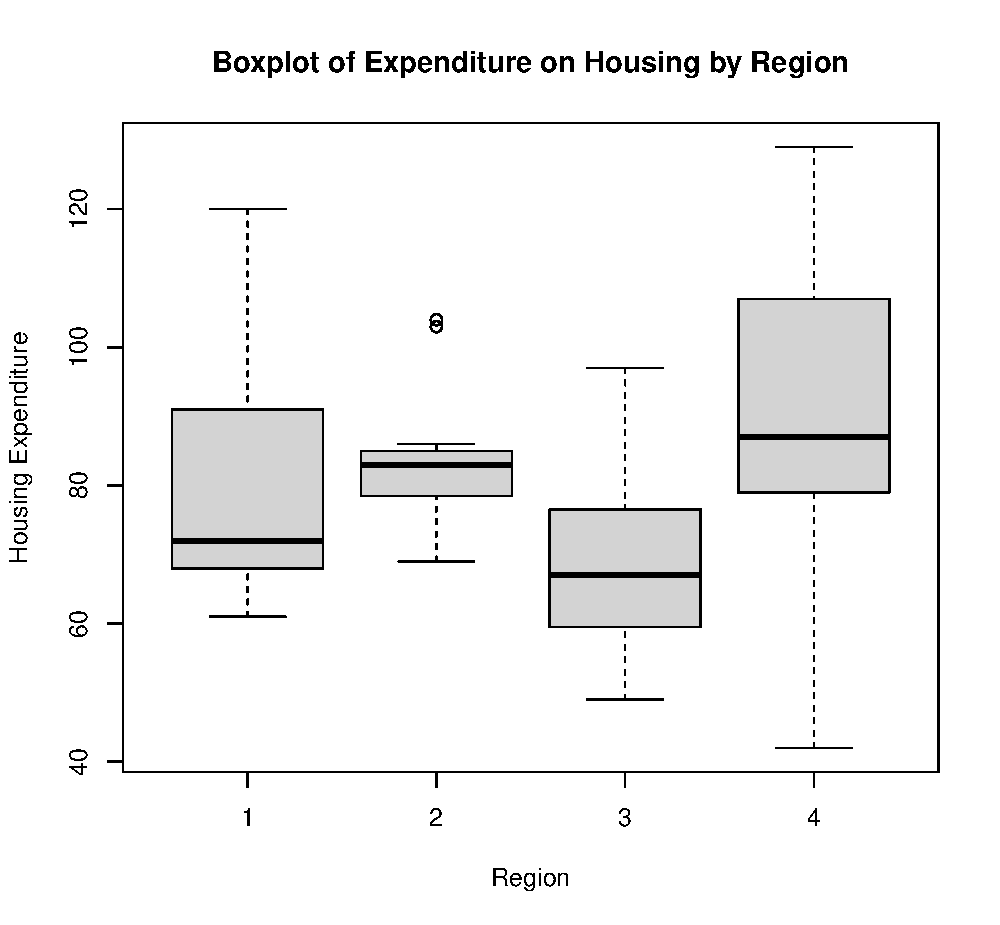
\includegraphics{Boxplot_Q2.2}
\end{center}
     
     Based on this boxplot we can see that region 4 (West) is the region with the highest average expenditure on housing.
     
     \subsection*{Part 3.}
     
     To plot the relationship between between Y and X1, I used the plot function in R.
     \begin{verbatim}
     	plot(expenditure$Y ~ expenditure$X1,
     	main="Scatterplot of Housing Expenditure by Personal Income",
     	xlab="Per Capita Personal Income",
     	ylab= "Expenditure on Housing")
     \end{verbatim}
     
     Which produced this scatterplot:
\begin{center}
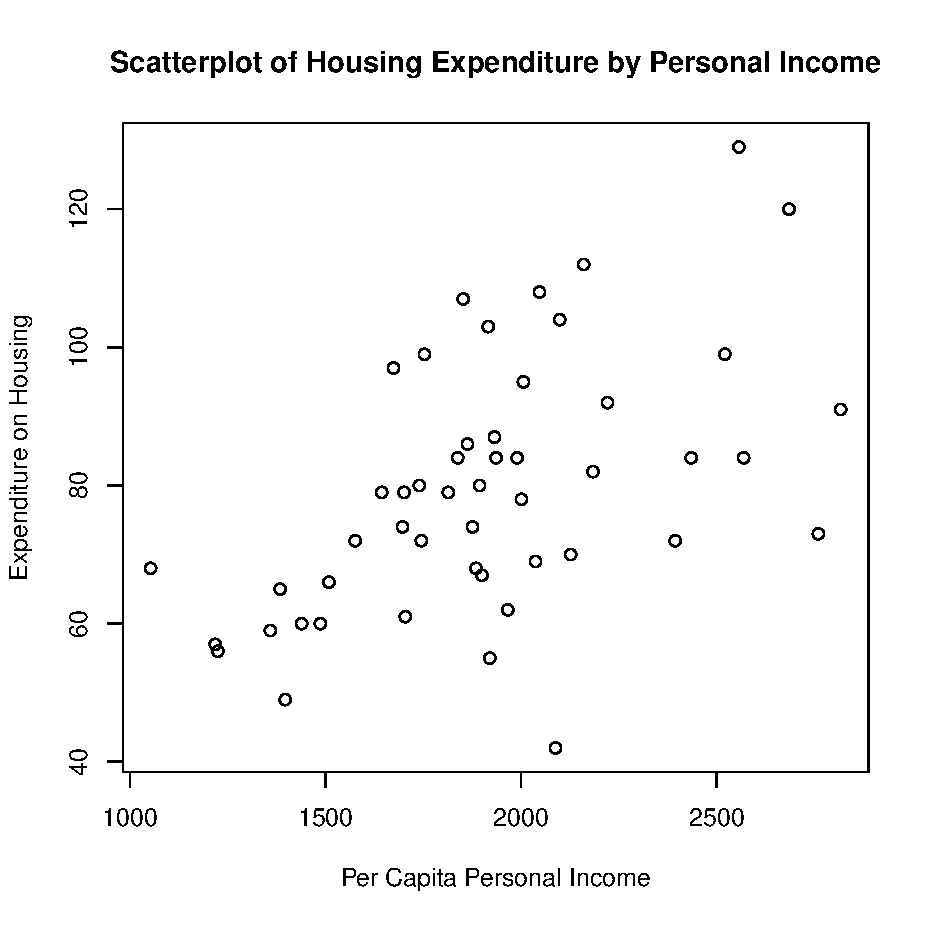
\includegraphics{incomeXexpenditureSPbase}
\end{center}

    To add a third variable (Region) to the plot with all the necessary parameters I wrote the following code:
    \begin{Verbatim}
    	colors <- c("red", "green", "blue", "orange")
    	plot(Y ~ X1,
    	data = expenditure,
    	main="Scatterplot of Housing Expenditure by Personal Income",
    	xlab="Per Capita Personal Income",
    	ylab= "Expenditure on Housing",
    	pch=expenditure$Region,
    	col= colors[expenditure$Region],
    	cex=1)
    	legend("right", legend = c("Northeast", "North Central", "South", "West"), 
    	pch = 1:4,  
    	col = colors,  
    	title = "Region")
    \end{Verbatim}
    
    Which produced this modified version of the scatterplot with a ledger to identify the regions by color and symbol:
\begin{center}
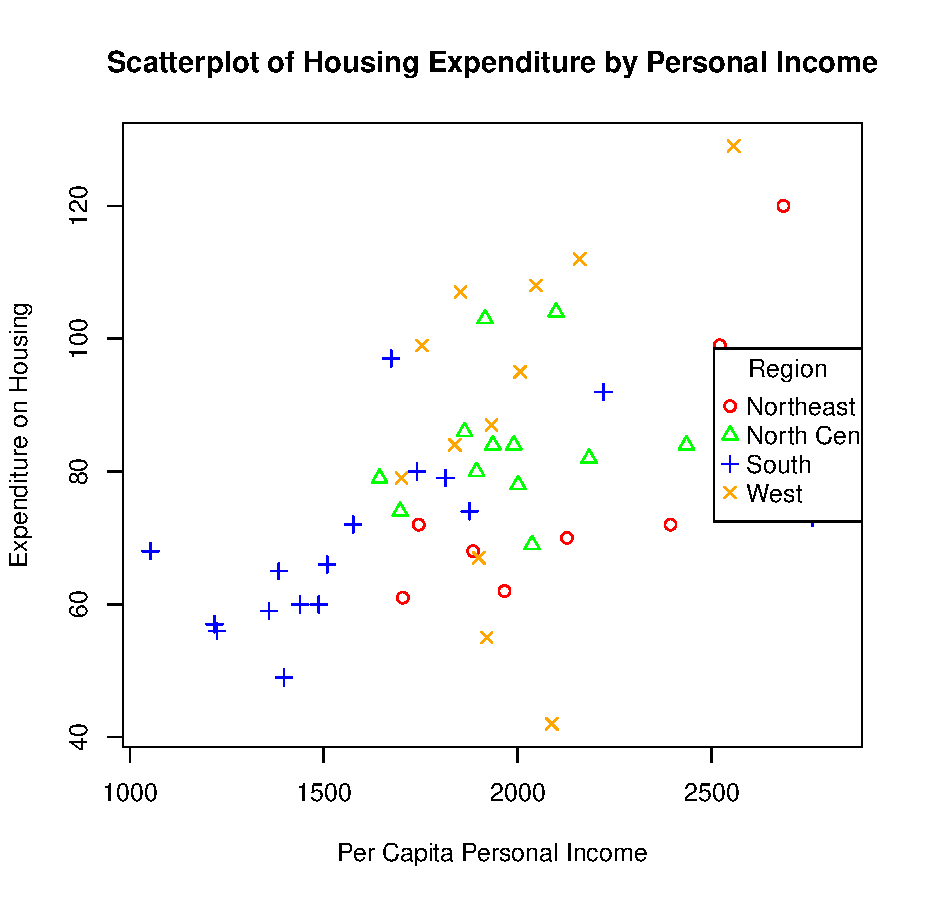
\includegraphics{Final_Scatter_Plot_Resized}
\end{center} 

\section*{Bibliography:}
\begin{enumerate}
	\item https://www.youtube.com/watch?v=zxp9pKIToWk
	\item https://www.geeksforgeeks.org/how-to-make-a-scatter-plot-matrix-in-r/
	\item https://www.datacamp.com/tutorial/t-tests-r-tutorial
	\item Statistical Methods for the Social Sciences, Fourth Edition.
	\item https://www.tutorialspoint.com/how-to-extract-the-p-value-from-t-test-in-r
	\item Tutorial material provided by Hannah Frank.
\end{enumerate}


     
     
     
\end{document}